% ASGARD/Loki draft (verified numbers, humanized)
\section{The QMMF Architecture}
\label{sec:method}

\begin{figure*}[tp]
\centering
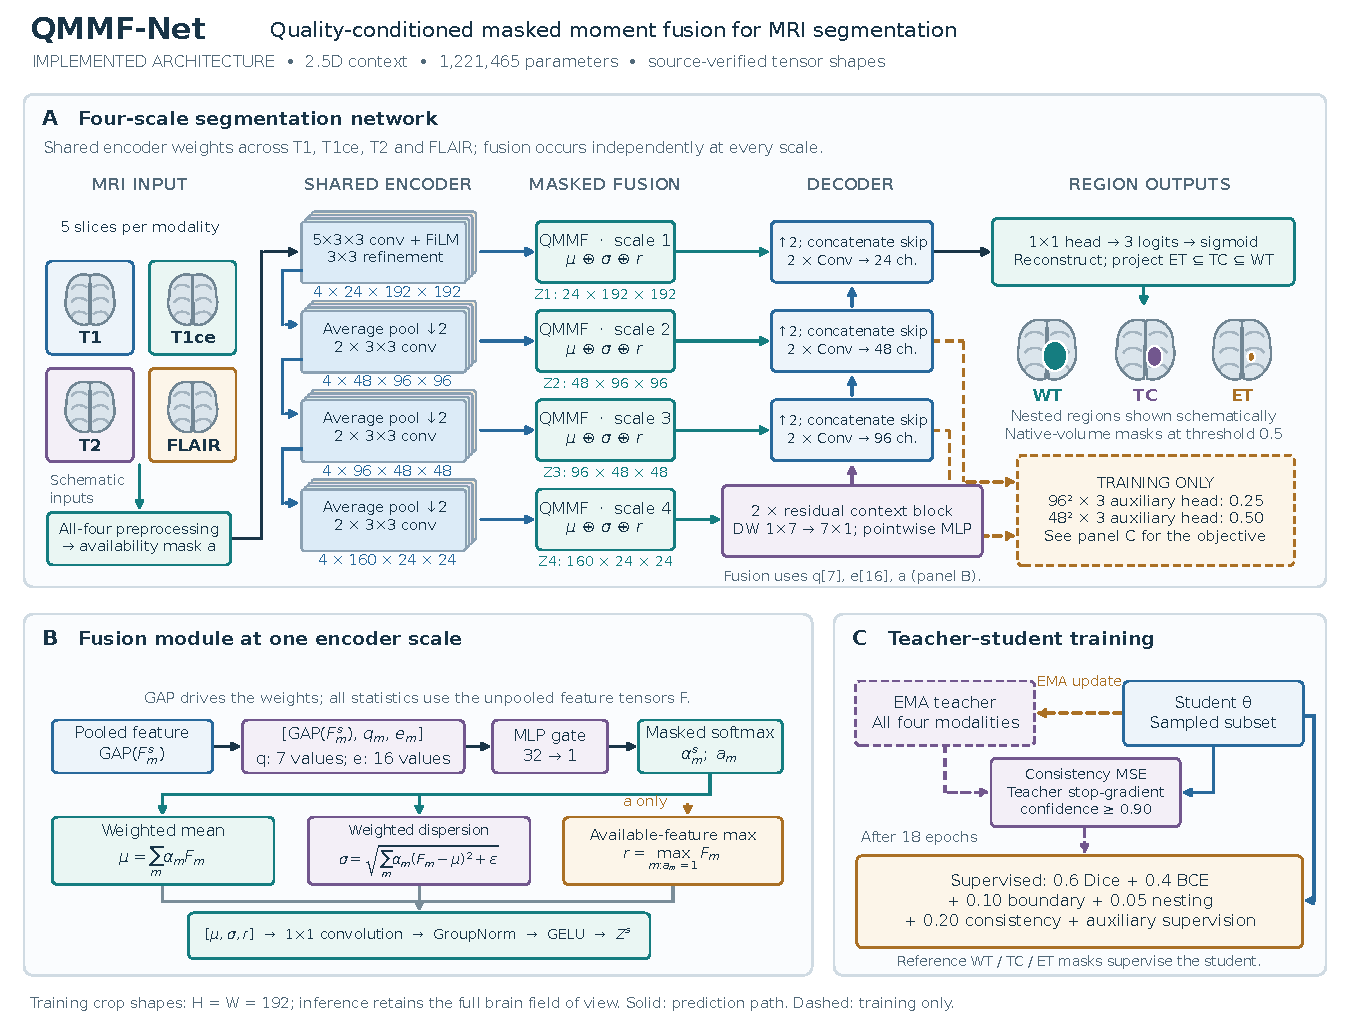
\includegraphics[width=\textwidth]{figures/qmmf_architecture.pdf}
\caption{Implemented quality-conditioned masked moment-fusion network. (A)~Five-slice windows from T1, T1ce, T2 and FLAIR pass through a modality-shared encoder; a learned modality embedding conditions the shared stem through FiLM. Per-modality features at four spatial scales are fused independently, fused features feed the decoder skips and a bottleneck with two factorised large-kernel residual blocks, and bilinear decoder stages predict overlapping WT/TC/ET outputs. (B)~A gate uses pooled features, seven quality proxies and modality identity to weight available inputs; fusion concatenates weighted mean, weighted dispersion and availability-only maximum. (C)~Training adds an EMA teacher with complete-modality inputs, confidence-masked subset consistency and two auxiliary heads (dashed, training-only). Shapes describe the 192$\times$192 training crop; anatomical icons are schematic.}
\label{fig:arch}
\end{figure*}

\begin{figure}[htbp]
\centering
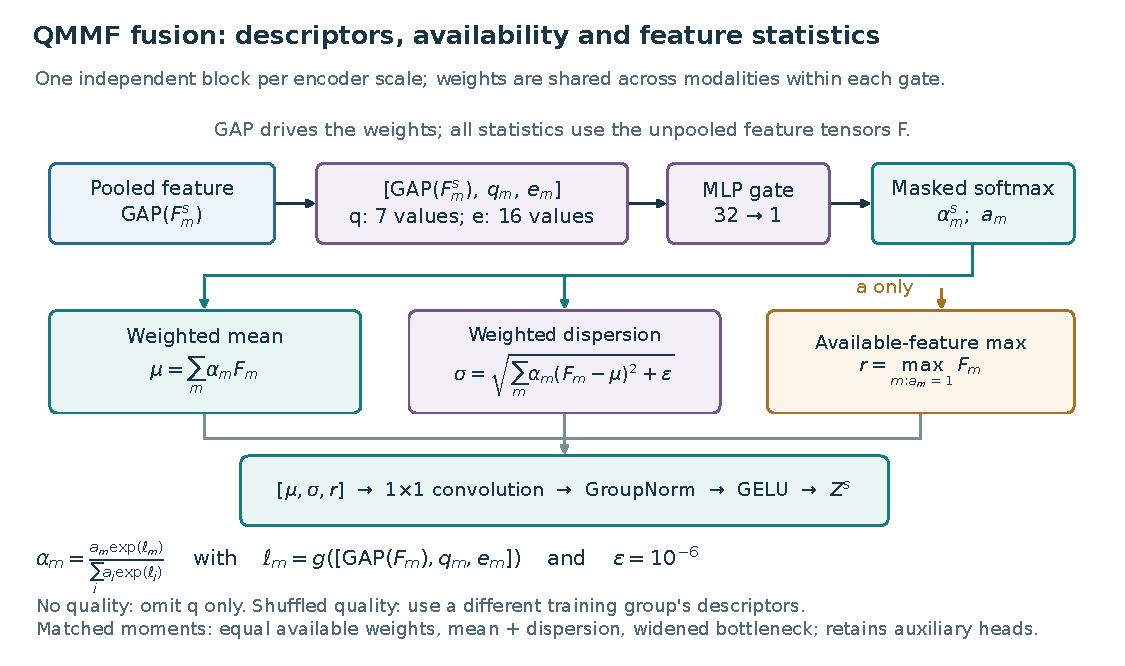
\includegraphics[width=\columnwidth]{figures/qmmf_fusion_detail.pdf}
\caption{Fusion detail and component controls. Pooled features determine one scalar gate weight per modality and scale; the three feature statistics act on the unpooled feature tensors. The maximum uses the availability mask and not the learned quality weights; the square-root variance branch uses $\epsilon=10^{-6}$. The no-quality control omits the quality descriptor from the gate; the shuffled-quality control substitutes descriptors donated by a different training group.}
\label{fig:fusion}
\end{figure}

The network receives images of shape $[B,4,5,H,W]$ with availability $[B,4]$ and quality descriptors $[B,4,7]$; $H{=}W{=}192$ for the recorded training crop. A shared five-slice stem---a $5{\times}3{\times}3$ convolution that collapses slice depth, GroupNorm, GELU, modality-identity FiLM and a $3{\times}3$ refinement---is applied to each modality by flattening the batch and modality axes, and encoded modality features remain separate until fusion. A four-scale encoder with widths 24/48/96/160 produces per-modality features that are fused independently at every scale; fused features feed the decoder skips and a bottleneck processed by two residual blocks of depthwise $1{\times}7$ and $7{\times}1$ convolutions with GroupNorm, a pointwise MLP with expansion two, and a LayerScale initialised at 0.01. The context block is convolutional, with no attention. Decoder stages upsample bilinearly (no transposed convolution), reduce channels with $1{\times}1$ convolutions, concatenate fused skips, and produce three overlapping sigmoid outputs for whole tumour (WT), tumour core (TC) and enhancing tumour (ET). The implementation has 1{,}221{,}465 parameters including two training-only auxiliary heads; a synthetic forward pass verifies every shape against the frozen configuration.

\paragraph{Quality-conditioned gate.}
For scale $s$ and modality $m$, let $F_m$ be the feature map, $q_m\in\mathbb{R}^7$ the quality descriptor, $e_m\in\mathbb{R}^{16}$ the learned modality embedding and $a_m$ the availability indicator (scale superscripts suppressed):
\begin{align}
\ell_m &= \mathrm{MLP}_s\!\big(\mathrm{concat}\big(\mathrm{GAP}(F_m),\,q_m,\,e_m\big)\big),\\
\alpha_m &= a_m\,\exp(\ell_m)\Big/\textstyle\sum_j a_j\exp(\ell_j),\\
\mu &= \textstyle\sum_m \alpha_m F_m,\qquad
\sigma = \sqrt{\textstyle\sum_m \alpha_m (F_m-\mu)^2 + 10^{-6}},\\
r &= \max_{m:\,a_m=1} F_m,\\
Z &= \mathrm{GELU}\!\big(\mathrm{GroupNorm}(\mathrm{Conv}_{1\times1}([\mu;\sigma;r]))\big).
\end{align}
The gate MLP has a 32-unit hidden layer with GELU and a scalar, bias-free output; logits are masked, absent weights zeroed, and weights renormalised over available modalities. Moment reductions run in float32. The maximum branch is availability-weighted, not quality-weighted. Fusion projects the concatenation with a $1{\times}1$ convolution, GroupNorm and GELU. The seven proxies and their measurements appear in Table~\ref{tab:proxies}.

\begin{table}[t]
\centering
\caption{The seven quality proxies, computed on complete preprocessed volumes and cached before augmentation. Training uses within-group medians, then fits per-modality medians and interquartile ranges across training groups, clipped to $\pm5$. These proxies are not validated acquisition-quality scores.}
\label{tab:proxies}
\scriptsize
\begin{tabular}{lp{5.4cm}}
\toprule
Proxy & Measurement \\
\midrule
snr\_proxy & foreground MAD divided by background MAD, with a numerical floor \\
coefficient\_variation & foreground SD divided by $|$mean$|+\epsilon$ \\
entropy & normalised entropy of a clipped 64-bin intensity histogram \\
robust\_dynamic\_range & foreground 95th--5th percentile range divided by MAD \\
zero\_support\_fraction & near-zero fraction within the chosen brain support \\
high\_frequency\_energy & mean gradient magnitude divided by MAD \\
center\_of\_mass\_shift & positive-intensity centroid displacement from the support centroid, normalised by volume extent \\
\bottomrule
\end{tabular}
\end{table}

\paragraph{Training and inference.}
The objective combines $0.6$ soft-Dice and $0.4$ BCE, plus boundary ($0.10$), nesting ($0.05$), consistency ($0.20$) and auxiliary losses ($0.50$ at $48{\times}48$, $0.25$ at $96{\times}96$):
\begin{align*}
\mathcal{L} &= \mathcal{L}_{\mathrm{seg}} + 0.10\,\mathcal{L}_{\mathrm{bnd}} + 0.05\,\mathcal{L}_{\mathrm{nest}}
 + 0.20\,\mathcal{L}_{\mathrm{cons}} + \mathcal{L}_{\mathrm{aux}},\\
\mathcal{L}_{\mathrm{cons}} &= \mathrm{mean}\big((p_s-p_t)^2 \;\text{where}\; \max(p_t,1-p_t)\ge 0.90\big).
\end{align*}
An EMA teacher receives the corresponding complete-modality window with all-one availability; its decay is scheduled from 0.99 to 0.999, gradients do not flow through it, and consistency activates at zero-based epoch 18 of 120, matching a 15\% warmup. At inference, each window predicts its central slice; ordered predictions restore the cropped brain grid, nested probabilities are projected ($\mathrm{TC}\le\mathrm{WT}$, $\mathrm{ET}\le\mathrm{TC}$), the crop is restored to native-volume geometry, and masks threshold at 0.5. The evaluated checkpoint is the selected student, not the EMA teacher; auxiliary heads are absent from the prediction path. Missingness is simulated by masking channels after complete four-channel preprocessing, including support and crop construction.

